\documentclass{standalone}
\usepackage{tikz}
\usepackage{ctex,siunitx}
\setCJKmainfont{Noto Serif CJK SC}
\usepackage{tkz-euclide}
\usepackage{amsmath}
\usetikzlibrary{patterns, calc}
\usetikzlibrary {decorations.pathmorphing, decorations.pathreplacing, decorations.shapes,}
\begin{document}
\small
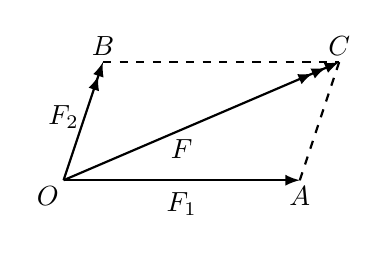
\begin{tikzpicture}[>=latex, thick,scale=1]
  % \useasboundingbox(-1,-0.75)rectangle(3.7,1.4);
  \draw [->>] (0,0)--(0.5, 1.5);
  \draw [->] (0,0)--(3, 0);
  \draw [dashed, thick] (0.5, 1.5)--(3.5, 1.5);
  \draw [->>>] (0,0)--(3.5, 1.5);
  \draw [dashed, thick] (3, 0)--(3.5, 1.5);
  \node at (-.2, -0.2){$O$};
  \node at (3, -0.2){$A$};
  \node at (.5, 1.7){$B$};
  \node at (3.5, 1.7){$C$};
  \node at (1.5, -.3){$F_1$};
  \node at (0, 0.8){$F_2$};
  \node at (1.5, 0.4){$F$};
\end{tikzpicture}
\end{document}